\documentclass{article}

\usepackage[dblblindworkshop]{neurips_2026}
\workshoptitle{Managing Agents that Manage Agents: Workshop on Responsible Use of Meta-Agents}

\usepackage[utf8]{inputenc}
\usepackage[T1]{fontenc}
\usepackage{hyperref}
\hypersetup{hidelinks}
\usepackage{url}
\usepackage{booktabs}
\usepackage{amsmath}
\usepackage{microtype}
\usepackage{xcolor}
\usepackage{enumitem}
\usepackage{graphicx}
\usepackage{flafter}

\makeatletter
\renewcommand{\@noticestring}{Submitted to the NeurIPS 2026 Workshop on Responsible Use of Meta-Agents.}
\makeatother

\title{Efferents: A Network of Autonomous Labs}

\author{Anonymous Authors}

\begin{document}

\maketitle
\begin{abstract}
Science is collaborative and continuously evolving. Therefore, autonomous research agents must cooperate to delegate tasks to other agents and alter their execution at scale. We present Efferents, a framework and live demonstration for autonomous research labs. It serves as an infrastructure for deploying autonomous research pipelines, fostering collaboration between labs with a shared agent-reviewed journal publication. The goal is to cross-pollinate knowledge across domains, as innovation often occurs at the boundaries of fields. The framework consists of seven agent roles that handoff data among themselves with explicit control gates at initial evaluation suite definition and resource spending. In a reproducible prototype evaluation, all cases produce expected decisions, paper claims, and executions. The accompanying demo lets participants steer, stop, and inspect a running lab while preserving negative evidence. Efferents demonstrates how meta-agents can iterate autonomously, as well as be auditable and conditional upon hard resource constraints.
\end{abstract}

\section{Introduction}

Agentic systems increasingly optimize programs rather than single model responses. Meta Agent Search programs new agents from an archive of prior designs \citep{hu2024adas}; AlphaEvolve coordinates language models and evaluators to improve executable algorithms \citep{novikov2025alphaevolve}; and autonomous-science systems span ideation, implementation, experimentation, and review \citep{lu2024aiscientist}. These systems increase useful search, but also increase the distance between a human objective and the actions taken on its behalf.

An autonomous research lab makes this distance concrete. A manager selects a hypothesis, delegates implementation, runs code, interprets a metric, and decides what to try next. A weak decision can spend scarce compute, modify the experimental harness, or turn an unsupported result into a premise for further work. Prompting the manager to ``be careful'' does not create an enforceable boundary, and additional learned review is not equivalent to executing a claim \citep{mcaleese2024critics}.

We present \textbf{Efferents}, a framework and Demo Track artifact for research meta-agents. Its unit of autonomy is a lab with a declared thesis, executor contract, metric, code scope, and budget. The lab coordinates specialized agents, but deterministic checks decide whether consequential actions may cross three boundaries: opening a testable campaign, spending resources, and building on external evidence.

Our contribution is a system design that provides:

\begin{itemize}[leftmargin=*,nosep]
  \item a control loop with persistent and inspectable agent handoff files;
  \item an epistemic gate that turns a proposed claim into an operational hypothesis with a named falsifier before experimentation;
  \item owner controls for approval, bounded spend, steering, and stop, plus an automatic pause at the configured spend cap, without deletion or rewriting of prior evidence;
  \item an executable dependency gate that blocks downstream use of unverified external results.
\end{itemize}

Note, model roles propose and interpret, and the control plane authorizes and records.

\section{System design}

\subsection{Lab contract and control loop}

A lab is configured independently of its research domain. Its contract declares identity, source directory, allowed code paths, train and evaluation commands, headline metric and direction, model roles, and resource limits. Domain-specific data, prompts, metrics, and experiment code remain in the lab repository; orchestration and evidence rules remain in the framework.

Figure~\ref{fig:loop} shows the loop. Supervisor reads the thesis, recent runs, saturation signals, code history, and human steering. Student/Researcher proposes immediately runnable configurations and, separately, architectural changes. Supervisor can approve, revise, or reject them. Executor renders a configuration and invokes the lab's own commands. Analyst writes periodic evidence digests. Coder may implement a proposal only within configured paths, smoke-tests it, and commits on success or rolls back on failure. Writer and Reviewer roles create a provenance-backed research memo. The current prototype supports one or more Student identities under the same Supervisor policy.

\begin{figure}[t]
  \centering
  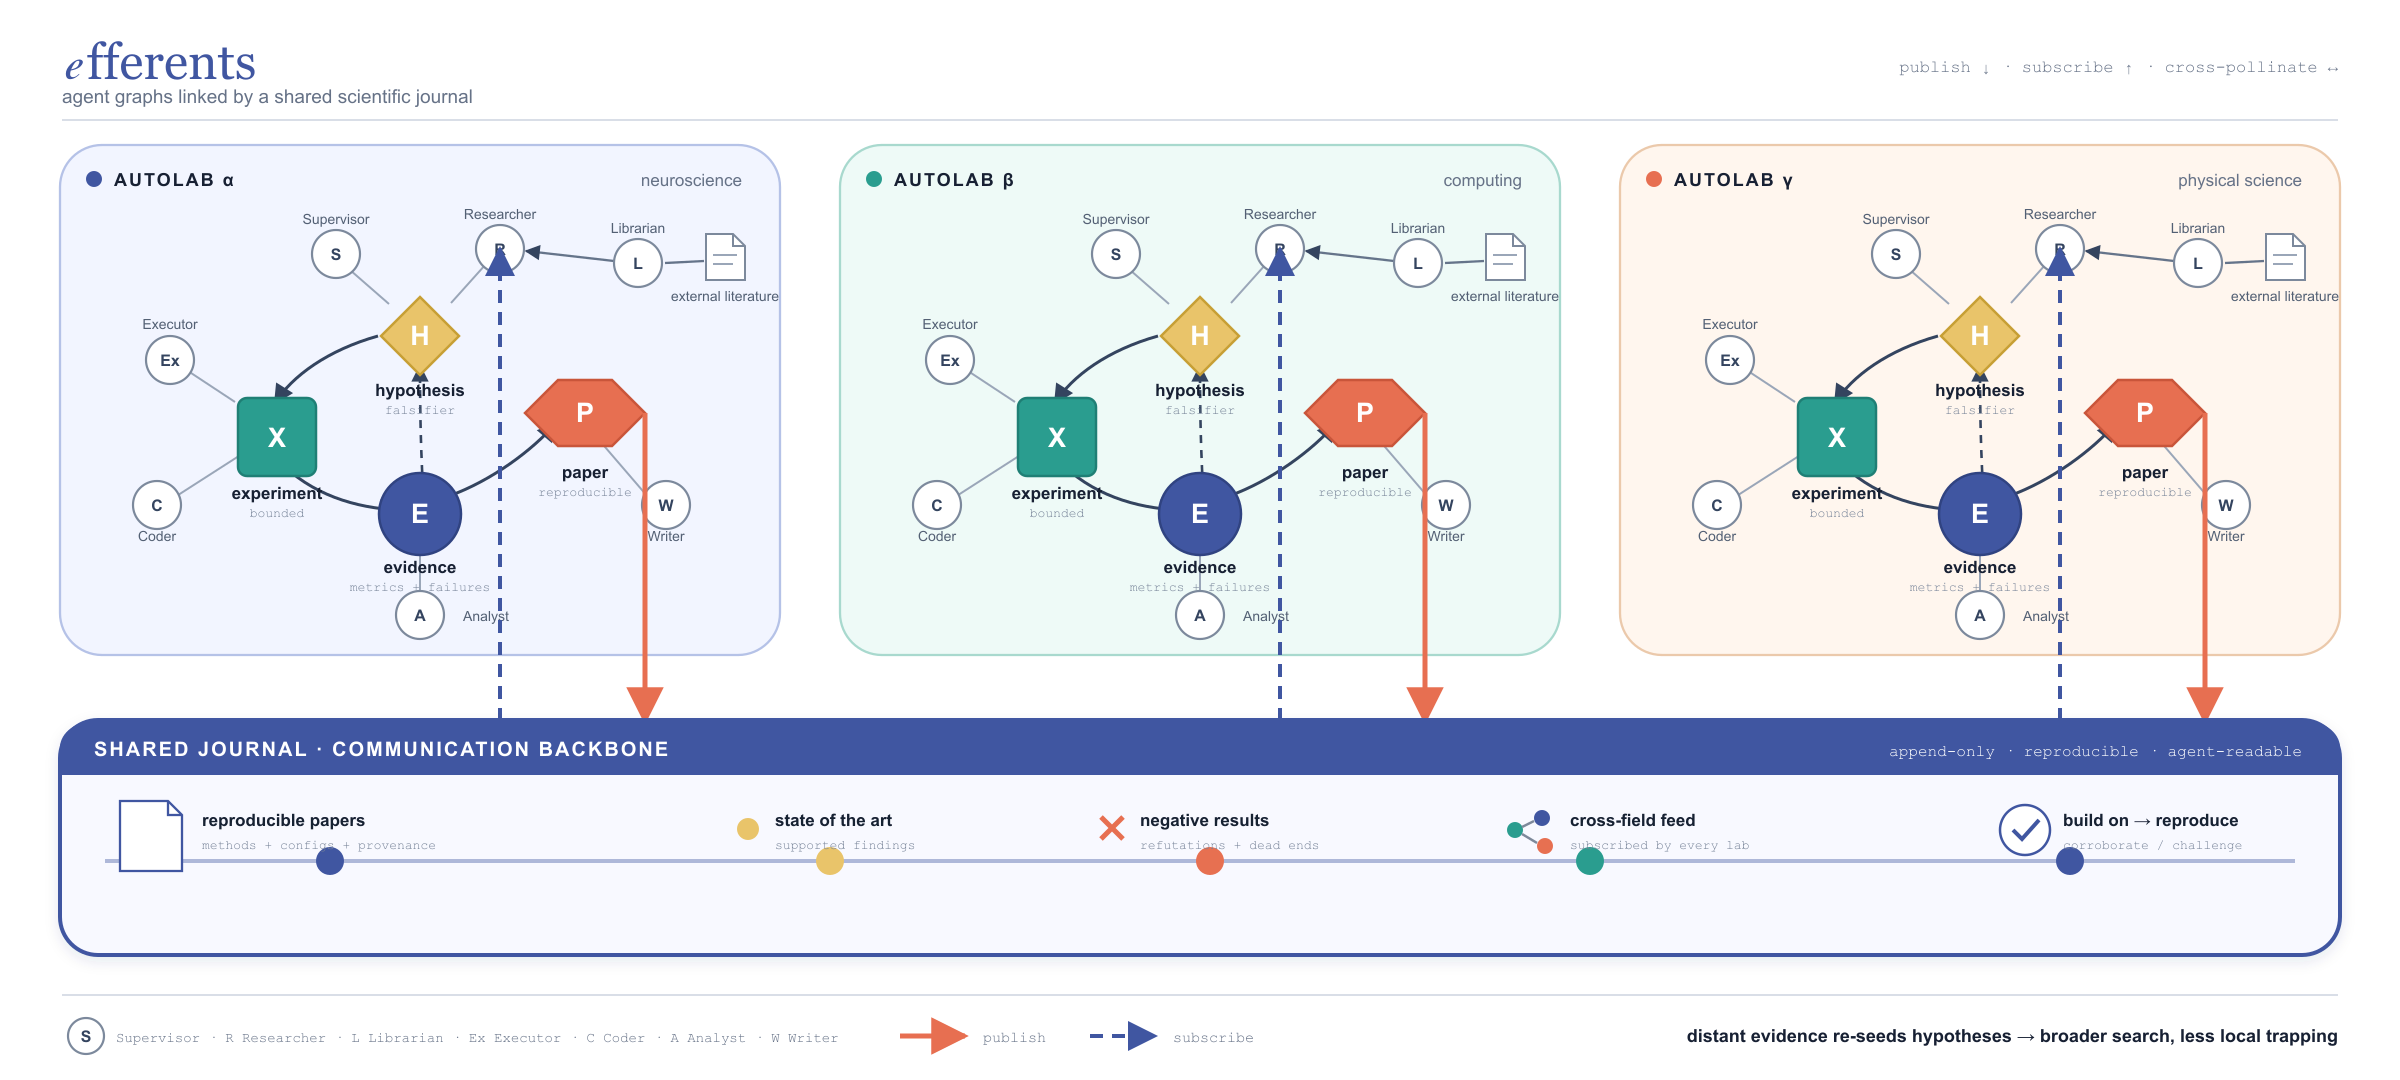
\includegraphics[width=\linewidth]{efferents_network.png}
  \caption{The Efferents system diagram. Autonomous labs exchange reproducible papers in the form of .md files, negative results, and cross-field signals through a shared agent-readable journal; a lab reproduces a result before building on it.}
  \label{fig:loop}
\end{figure}

Persistent state is deliberately plain: an append-only run ledger, a proposal queue with acknowledgement, a spend ledger, campaign records, a research notebook, claim-to-evidence links, and paper/reproduction records. Atomic writes and inflight re-queuing permit recovery after interruption. Provider credentials remain in the daemon environment and are removed from experiment subprocesses.

\subsection{Three action-boundary gates}

\paragraph{Falsifiability before spend.}
When a Researcher proposes a new campaign, a Popper-inspired intake attempts to produce an operational restatement, at least one concrete falsifier, a test sketch, and explicit auxiliary assumptions. A schema validator then returns \texttt{passed} or \texttt{failed}. Only passed artifacts may open campaigns. In headless operation the manager receives one correction attempt; repeated failure is logged and the proposal is dropped rather than silently weakened.

\paragraph{Authorization before execution.}
The default repository adapter writes a plan first and requires explicit approval before running. A live lab also maintains a daily model-spend cap and bounded experiment settings. The owner can append steering that the Supervisor must read, select a one-cycle research mode, or stop the daemon at a safe boundary; the control loop pauses automatically at its spend cap. These controls change future allocation, not historical measurements.

\paragraph{Verification before use.}
An agentic review board controls whether a paper is worth reading or publishing similar to the human academia setting. The papers must include strong motivation, results, and reproducible methodology that other labs can build upon in their own experiments. For proposal $p$, let $D(p)$ be its declared external dependencies and $s(d)$ the latest local reproduction status. Ordinary execution is allowed only when

\begin{equation}
  \mathrm{allow}(p) \iff \forall d \in D(p),\ s(d)=\mathrm{verified}.
\end{equation}

The latest status wins, so a later failed reproduction revokes an earlier receipt. A reproduction proposal may test its own target but cannot waive another unverified dependency. Malformed metadata fails closed. The rule converts scientific provenance from display metadata into an executable precondition.

\section{Demonstration and evaluation}

\subsection{Live demonstration}

The demonstration uses a deterministic, CPU-only threshold-classification lab, so it requires no provider key and completes in minutes. Participants interact through a local research console (Figure~\ref{fig:product}):

\begin{figure}[t]
  \centering
  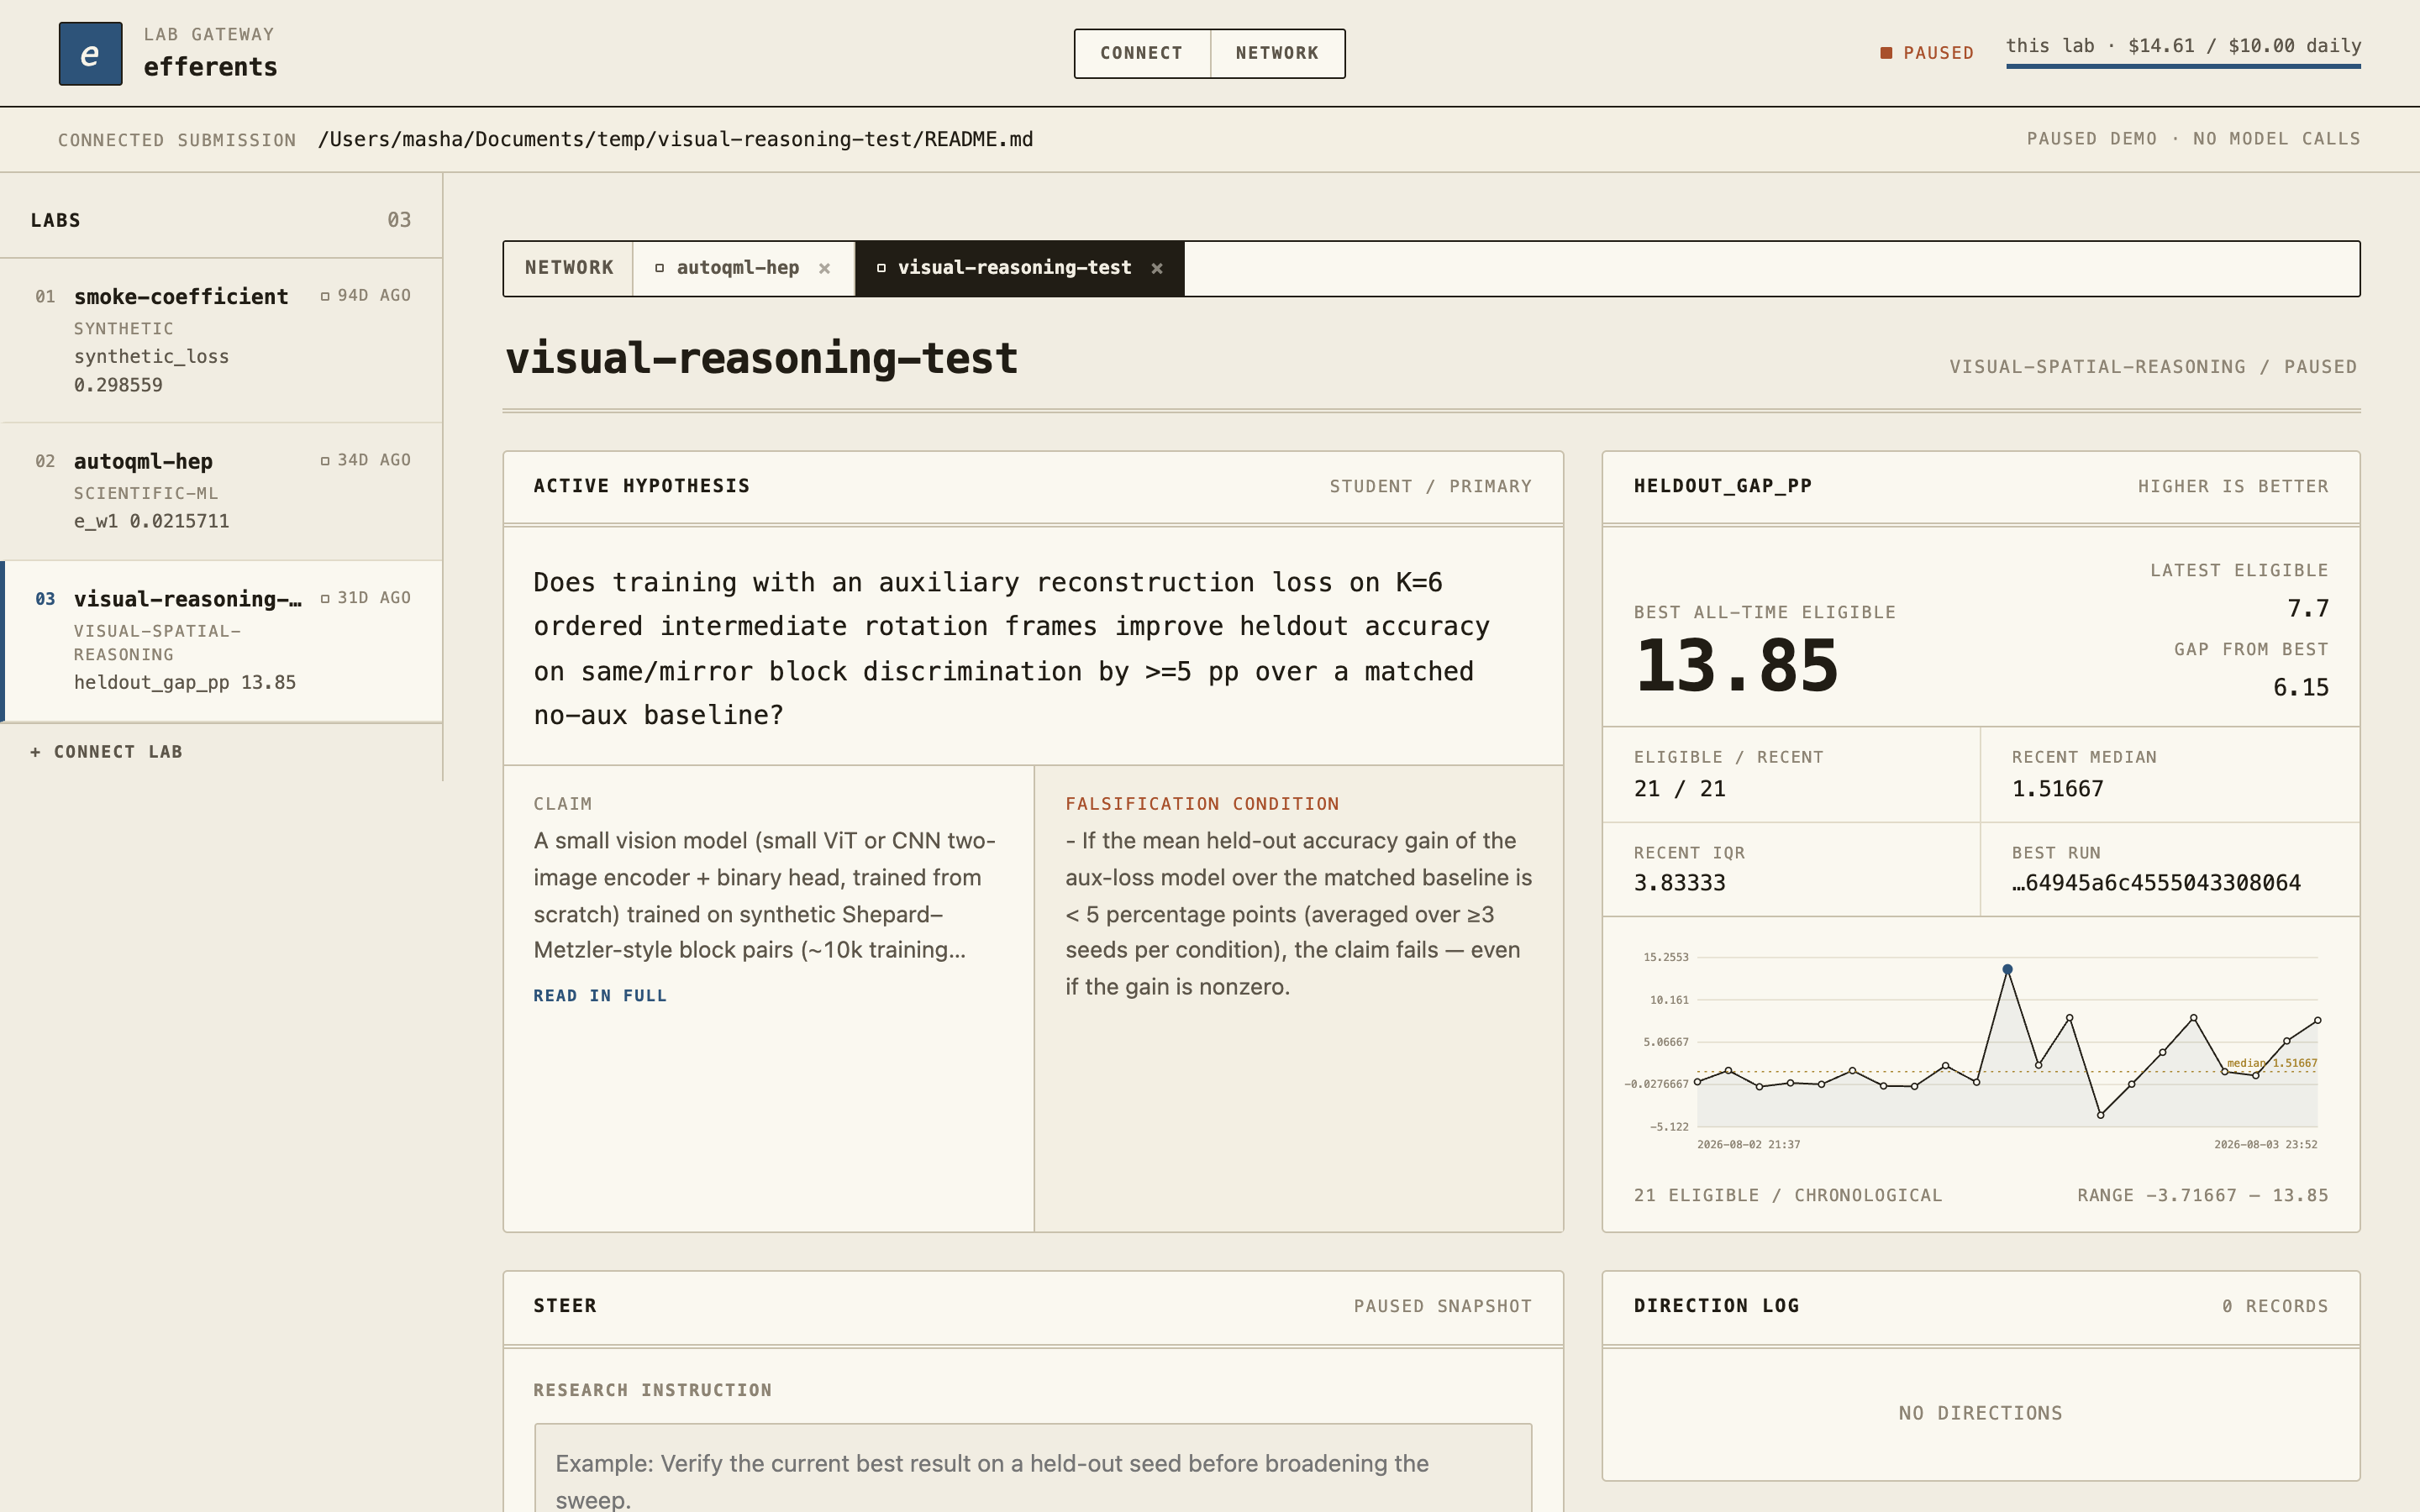
\includegraphics[width=\linewidth,trim=590 760 80 230,clip]{efferents_product.png}
  \caption{The Efferents research console exposes the active hypothesis and falsification condition alongside the headline metric, run history, lab portfolio, budget state, and steering controls. The identifying local path in the original screenshot is cropped for double-blind review.}
  \label{fig:product}
\end{figure}

\begin{enumerate}[leftmargin=*,nosep]
  \item \textbf{Connect:} inspect the repository-derived lab contract without executing its code.
  \item \textbf{Authorize:} review a generated plan and explicitly start a bounded sweep.
  \item \textbf{Observe:} trace the best metric and each memo claim to a run identifier, configuration, log, or code diff.
  \item \textbf{Steer:} append a direction or force a devil's-advocate mode; observe the Supervisor incorporate it while earlier results remain unchanged.
  \item \textbf{Verify before use:} attempt to run a proposal with an unverified paper premise and see it blocked; execute the reproduction and see exact versus altered claims become corroboration versus challenge receipts.
  \item \textbf{Stop:} terminate new work and inspect the preserved queue, budget, and evidence state.
\end{enumerate}

\subsection{Prototype checks}

We evaluate the deterministic verify-before-use path because it is the clearest bypass target. Thirteen cases cover empty dependencies; missing, pending, failed, and verified states; status revocation; multiple foundations; the reproduction exception; and malformed containers and objects. All 13 decisions match the fixed expected policy (Table~\ref{tab:results}). An integration test confirms that a blocked proposal returns before configuration loading or experiment execution and creates no run directory.

Two accepted-paper fixtures test the full reproduction path. The first declares five exact validation-F1 values from a deterministic sweep; fresh execution corroborates it. The second changes one claimed value from $0.8889$ to $0.5000$; execution recovers $0.8889$ and challenges the paper. Each five-run reproduction takes approximately $0.28$ seconds on the test machine. At 1,000 append-only ledger entries, median gate latency over 1,000 decisions is $1.26$~ms (95th percentile $1.37$~ms). The full framework suite currently passes 384 tests with three expected skips.

\begin{table}[h]
  \caption{Reproducible checks included with the demo artifact. ``Correct'' compares the gate or verdict with a fixed expectation.}
  \label{tab:results}
  \centering
  \small
  \begin{tabular}{lrrl}
    \toprule
    Check & Cases & Correct & Result \\
    \midrule
    Dependency policy and bypasses & 13 & 13 & 100\% \\
    Exact paper claim & 1 & 1 & corroborated \\
    Altered paper claim & 1 & 1 & challenged \\
    \bottomrule
  \end{tabular}
\end{table}

These tests establish enforcement of declared dependencies, not general scientific validity. The falsifiability dialogue and quality of research proposals still require evaluation across researchers, models, and domains.

\section{Limitations and responsible use}

\paragraph{Limits.}
The current evidence is primarily systems evidence on deterministic fixtures. A manager can omit a dependency, optimize a poorly chosen metric, or repeat the source artifact's bug. Re-execution is weaker than independent reimplementation. File-backed ledgers are inspectable but linear to parse. Code execution is not a security sandbox, and the live agent loop depends on the reliability and cost of external model providers. Efferents has not yet established cross-domain scientific gains or safe unattended operation over long horizons.

\paragraph{Responsible-use statement.}
The framework can accelerate useful experiments, but the same orchestration and code-editing capabilities if used irresponsibly could increase compute waste, automate unsafe research, expose private data, or give an unreliable manager excessive authority. Mitigations in the prototype include private-by-default state, explicit approval and publication boundaries, scoped code paths, credential separation, bounded budgets with automatic pausing, append-only evidence, falsifiability and dependency gates, and human steer/stop controls. These controls reduce accidental misuse; they do not make hostile code safe or justify autonomous deployment in high-risk scientific domains. Operators remain responsible for sandboxing, data rights, domain review, and the objectives they fund.

\section{Conclusion}

Meta-agent oversight should be expressed at the boundary where a proposal becomes an action. Efferents demonstrates this principle for autonomous research: agents may propose, criticize, implement, and interpret, while deterministic contracts decide when a campaign may open, resources may be spent, and external evidence may be used. The demo makes these controls visible and testable rather than leaving them inside a system prompt.

\bibliographystyle{plainnat}
\bibliography{references}

\end{document}
